\begin{figure}
    \subfloat[Number of SPPF nodes.]{
        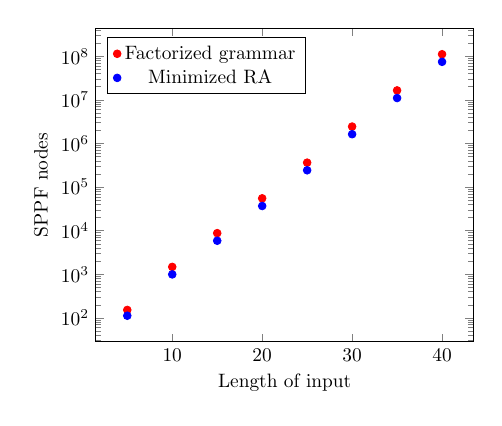
\begin{tikzpicture}[scale=0.7]
        \begin{axis}[
        legend pos = north west,
        xlabel = {Length of input},
        ylabel = {SPPF nodes},
        ymode=log
        ]
        \addplot [only marks, red] coordinates {
            (5,152) (10,1475) (15,8762) (20,55087) (25,362619) (30,2435360) (35,16441390) (40,111127244)
        };
        \addplot [only marks, blue] coordinates {
            (5,112) (10,993) (15,5869) (20,36771) (25,242360) (30,1627957) (35,10991272) (40,74292078)
        };
        \legend{ 
            Factorized grammar, 
            Minimized RA
        };
        \end{axis}
        \end{tikzpicture}
        \label{fig:SPPFnodes}
    }
    ~
    \subfloat[Number of descriptors.]{
        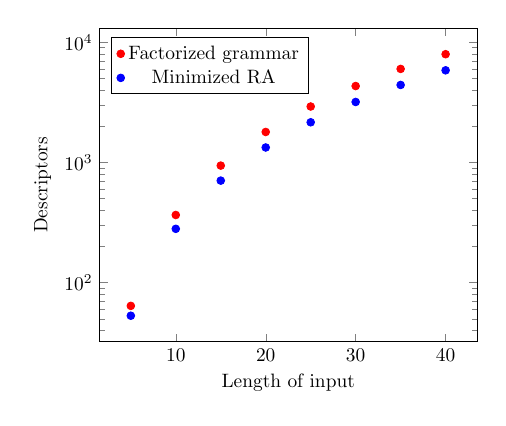
\begin{tikzpicture}[scale=0.7]
        \begin{axis}[
        legend pos = north west,
        xlabel = {Length of input},
        ylabel = {Descriptors},
        ymode=log
        ]
        \addplot [only marks, red] coordinates {
            (5,64) (10,365) (15,940) (20,1790) (25,2915) (30, 4315) (35,5990) (40,7940)
        };
        \addplot [only marks, blue] coordinates {
            (5,53) (10,280) (15,705) (20,1330) (25,2155) (30, 3180) (35, 4405) (40,5830)
        };
        \legend{ 
            Factorized grammar, 
            Minimized RA
        };
        \end{axis}
        \end{tikzpicture}
        \label{fig:Descriptors}
    }
    \caption{Experiments results(2).}
    \label{expPlots2}
\end{figure}